\FloatBarrier

\begin{figure}[h!]
	\centering
	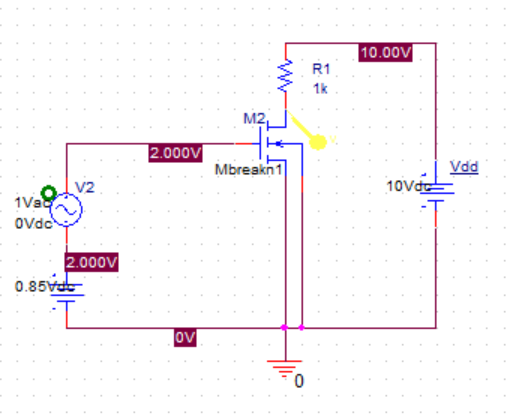
\includegraphics[scale=0.75]{../images/circuit2.PNG}
	\caption{}
	\label{fig:circuit2}
\end{figure}

\FloatBarrier

\FloatBarrier

\begin{figure}[h!]
	\centering
	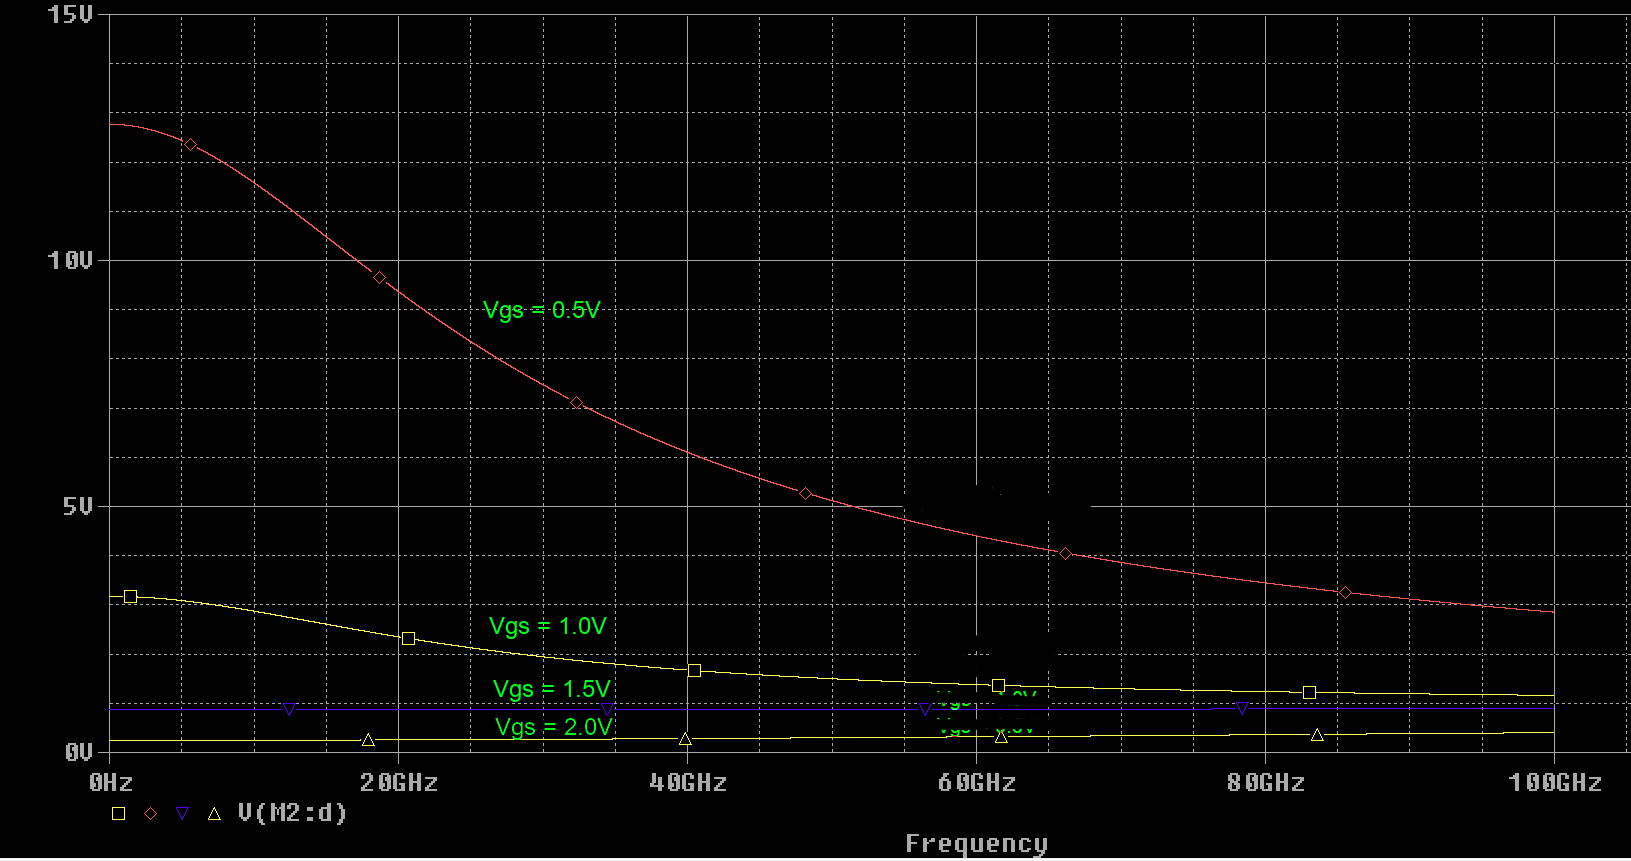
\includegraphics[scale=0.75]{../images/vout_vs_f.PNG}
	\caption{AC Sweep of Common-Source Amplifier}
	\label{fig:vout_vs_f}
\end{figure}

\FloatBarrier

Given the SPICE MOSFET model parameters, the NMOS's transconductance parameter $k_n$ is approximately $19.4 \frac{mA}{V^2}$. Its transconductance $g_m$ is given by $k_n V_{ov}$. $V_{ov}$ is simply the bias voltage at the gate minus the threshold voltage $V_T$. The threshold voltage is set to $0.362984$\si{\volt} in the MOSFET model.

\FloatBarrier

\begin{table}[h!]
	\centering
	\caption{}
	\label{tab:ss_gm}
	\csvautotabular{../tables/ss_gm.csv}
\end{table}

\FloatBarrier

The transconductance $g_m$ increases with $V_{GS}$ since more charge accumulate in the channel when the gate voltage is higher. Since the MOSFET's channel can support more charge, higher currents can flow for the same applied $V_{DS}$. The transconductance captures how well voltage applied to the MOSFET is converted to current, so the transconductance should be higher at higher $V_{GS}$ values. \\

The output resistance is given by $r_o = \frac{1}{\lambda I_D'}$. $\lambda$ is given as $0.02 V^{-1}$ in the SPICE model. $I_D'$ is the saturation current without taking channel-length modulation into account. So, $I_D' = \frac{k_n}{2} V_{ov}^2$. Therefore, the output resistance is given by:

\begin{equation}
	\label{eq:output_r}
	r_o = \frac{2}{\lambda k_n ( V_{GS} - V_T )^2}
\end{equation}

\FloatBarrier

\begin{table}[h!]
	\centering
	\caption{}
	\label{tab:ss_ro}
	\csvautotabular{../tables/ss_ro.csv}
\end{table}

\FloatBarrier

It has already been established that higher currents flow when $V_{GS}$ is higher. If this is the case, then if one were to calculate the resistance for a fixed $V_{DS}$ value, higher currents would flow whenever $V_{GS}$ is increased. So, the output resistance drops as $V_{GS}$ is increased since higher currents flow for the same applied voltage. \\

The open circuit small-signal gain of a common source amplifier is given by $A_{vo} = -g_m R_D$, where $R_D$ is the drain resistance. $R_D$ here is fixed, but $g_m$ increases with $V_{GS}$. So, the small-signal gain increases with increasing $V_{GS}$. If $V_{GS}$ is higher, then $g_m$ is higher, meaning the MOSFET more easily converts a voltage applied at the gate to a current flowing through the MOSFET. So, smaller variations in the gate voltage, lead to larger variations in the drain current. $V_{out}$ is directly related to the drain current because of the resistor in series with the MOSFET. So, smaller variations in the gate voltage lead to larger variations in the output voltage $V_{out}$ when one increases $V_{GS}$.

\FloatBarrier

\begin{figure}[h!]
	\centering
	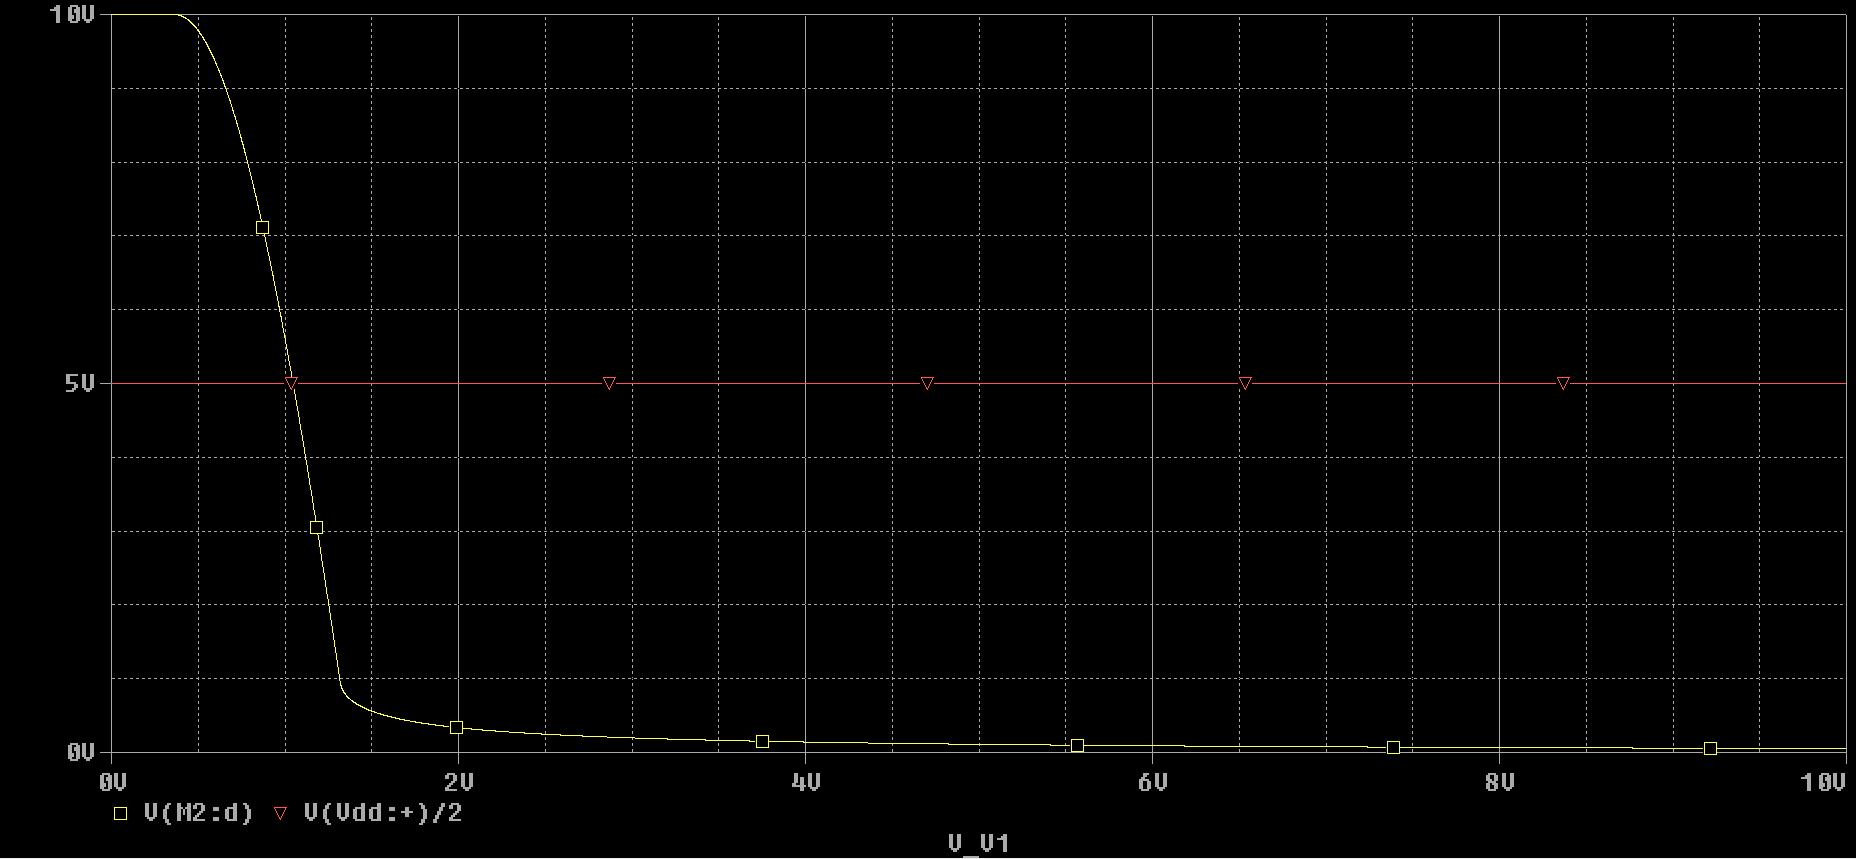
\includegraphics[scale=0.75]{../images/vout_vs_v3.PNG}
	\caption{DC Sweep}
	\label{fig:vout_vs_v3}
\end{figure}

\FloatBarrier

If $V_{GS}$ is biased at about $1$\si{\volt}, then the output voltage $V_{out}$ is biased at about $\frac{V_{DD}}{2}$, where $V_{DD} = 10$\si{\volt} is the supply voltage. As the input bias voltage at $V_{GS}$ is increased, the output bias voltage at $V_{out}$ decreases because of the inverting nature of the common source amplifier. If the amplifier is biased in the middle of the saturation region, which is where the steep downward slope in figure (\ref{fig:vout_vs_v3}) occurs, then varying the small-signal $V_{gs}$ linearly varies the output voltage $V_{out}$. This is because the slope, or $\frac{dV_{out}}{dV_{in}}$, is steepest in this region. So, the amplifier is most linear when it is biased here. If it is biased closer to cutoff region at lower voltages or the triode region at higher voltages, varying $V_{gs}$ could produce a clamped waveform at the output, meaning the gain is not constant, and the amplifier is not linear. \\
